\subsection{Backbone-NCA on Hippocampus}
\label{experiments:03.1.0:backbone_hippo:intro}
In this section, we come to our most commonly used setup and the most comprehensive results. 
As first setup for the robustness test, we choose the BackboneNCA (\autoref{methods:NCA:Models}) and the hippocampus dataset with spike and random noise augmentations as they have just been presented.

First, we will see in \autoref{experiments:03.1.1:backbone_hippo:spike_noise} that the DiceBceNQM improves the robustness to radiological noise compared to the DiceBCE 
by up to 7 points on the Dice when artifacts were sparse (''0.01'') in the dataset, and by up to 15 points on the Dice when no artifacts were present in the training dataset, and also leads to no degradation in all other tests in this setup.

In the subsequent parts, we present several approaches to improve this setup further. Of particular note are the speedup achieved by using pretrained models (\autoref{experiments:03.1.2:backbone_hippo:pretrained}) and a minimum stacksize of 2 (\autoref{experiments:03.1.3:backbone_hippo:stackSize}). With both approaches, we did not notice any loss of robustness gain due to the DiceBceNQM.

Then we introduce the hyperparameter alpha ($\alpha$) in \autoref{experiments:03.1.4:backbone_hippo:alpha}, which at a value of 2.0 increases robustness furthermore compared to DiceBceNQM without alpha by up to 4 points on the Dice.
Finally, in \autoref{experiments:03.1.x:FurtherNQMLosses} we come to the testing of alternative nonlinear loss functions with NQM, where especially the sqrtNQM (\autoref{experiments:03.1.7:backbone_hippo:sqrtNQM}) is a promising candidate, mainly because this loss shows equivalent robustness improvements, but should converge faster. However, speed tests in this regard were not part of this work.

%%% --- inputs ---
\subsubsection{Augmented Datasets}
\label{experiments:03.1.1:backbone_hippo:spike_noise}
To test how the DiceBceNQM (\autoref{experiments:02.1:diceBce+NQM}) performs on augmented data, we trained one model with the DiceBceNQM and one model with the DiceBCE for each spike and noise dataset, as well as the original dataset without augmentations. A total of 22 models. The results can be seen in \autoref{tab:03.1.1:DiceBCE+NQM_vs_DiceBCE_on_Noise} and \autoref{tab:03.1.1:DiceBCE+NQM_vs_DiceBCE_on_Spike}. We tested these models on all datasets of the series (i.e., all Spike or all Noise datasets as well as the original dataset). The models trained on the DiceBCE for each dataset serve as a baseline for the models trained on the DiceBceNQM. The test results of DiceBceNQM - Spike 1.0 are compared to the test results of DiceBCE - Spike 1.0, the test results of DiceBceNQM - Noise 1.0 are compared to the test results of DiceBCE - Noise 1.0, and so on. The models with DiceBceNQM perform significantly better than the models with DiceBCE alone. All models are better or no worse. The range goes from -1 to +15 on the Dice and is massively positive, and almost all values are positive. Also noteworthy are the vast improvements on the fully augmented data (Noise 1.0 and Spike 1.0) of the models trained on the original dataset, for Spike +9 points, for Noise +15, as well as the vast improvements for the Spike models trained on the sparsely augmented data (Spike 0.01) of +7 points on Spike. Noise has ''only'' +2 points here.

Therefore, using the DiceBceNQM improves robustness in this setting without adverse effects. First and foremost, a model trained with DiceBceNQM on the original dataset becomes much more robust on both spiked and noisy datasets than if trained with DiceBCE alone. Furthermore, the models trained on sparse augmented datasets (Spike 0.01 and Noise 0.01), as well as all others, also benefit from the DiceBceNQM, or at least are not degraded by it.

\begin{table}%[H]
    \centering
    \begin{tabular}{ll!{\vrule width 1.3pt}llllll}
        \toprule
        \multicolumn{2}{c!{\vrule width 1.3pt}}{model} &
        \multicolumn{5}{c}{\textbf{test dataset} (Dice $\uparrow$)}\\\midrule
        {\bfseries train loss} & \textbf{train set} & original & Spike 1.0 & Spike 0.3 & Spike 0.2 & Spike 0.1 & Spike 0.01\\\midrule[1.3pt]
        % ---
        DiceBCE     & original      & 0.879 & 0.574 & 0.793 & 0.791 & 0.841 & 0.880\\
        DiceBceNQM  & original      & 0.881 & 0.661 \textbf{+.09} & 0.812 +.02 & 0.811 +.02 & 0.858 +.02 & 0.881\\\rowcolor{BG}
        DiceBCE     & Spike 1.0     & 0.874 & 0.823 & 0.870 & 0.871 & 0.872 & 0.874\\\rowcolor{BG}
        DiceBceNQM  & Spike 1.0     & 0.873 & 0.814 -.01 & 0.870 & 0.866 -.01 & 0.872 & 0.873\\
        DiceBCE     & Spike 0.3     & 0.878 & 0.757 & 0.856 & 0.862 & 0.875 & 0.878\\
        DiceBceNQM  & Spike 0.3     & 0.879 & 0.769 +.01 & 0.861 +.01 & 0.864 & 0.873 & 0.878\\\rowcolor{BG}
        DiceBCE     & Spike 0.2     & 0.878 & 0.731 & 0.839 & 0.858 & 0.866 & 0.878\\\rowcolor{BG}
        DiceBceNQM  & Spike 0.2     & 0.879 & 0.744 +.01 & 0.837 & 0.864 +.01 & 0.868 & 0.879\\
        DiceBCE     & Spike 0.1     & 0.879 & 0.730 & 0.844 & 0.856 & 0.873 & 0.879\\
        DiceBceNQM  & Spike 0.1     & 0.880 & 0.755 +.03 & 0.851 +.01 & 0.866 +.01 & 0.874 & 0.880\\\rowcolor{BG}
        DiceBCE     & Spike 0.01    & 0.880 & 0.615 & 0.802 & 0.820 & 0.848 & 0.879\\\rowcolor{BG}
        DiceBceNQM  & Spike 0.01    & 0.880 & 0.685 \textbf{+.07} & 0.827 +.02 & 0.834 +.01 & 0.856 +.01 & 0.879\\\bottomrule
    \end{tabular}
    \caption{Backbone-NCA, hippocampus dataset \textbf{Augmented with Spikes} (\autoref{experiments:03.1.1:backbone_hippo:spike_noise}): Using the DiceBceNQM improves robustness in this setting without having any adverse effects. First and foremost, a model trained on the original dataset with the DiceBceNQM becomes much more robust on the Spiked Dataset than if trained on the DiceBCE alone.}
    \label{tab:03.1.1:DiceBCE+NQM_vs_DiceBCE_on_Spike}
\end{table}
\begin{table}%[H]
    \centering
    \begin{tabular}{ll!{\vrule width 1.3pt}llllll}
        \toprule
        \multicolumn{2}{c!{\vrule width 1.3pt}}{model} &
        \multicolumn{5}{c}{\textbf{test dataset} (Dice $\uparrow$)}\\\midrule
        {\bfseries train loss} & \textbf{train set} & original & Noise 1.0 & Noise 0.3 & Noise 0.2 & Noise 0.1 & Noise 0.01\\\midrule[1.3pt]
        % ---
        DiceBCE     & original            & 0.880 & 0.549 & 0.798 & 0.823 & 0.859 & 0.880\\
        DiceBceNQM  & original            & 0.881 & 0.703 \textbf{+.15} & 0.839 +.04 & 0.852 +.03 & 0.871 +.01 & 0.881\\\rowcolor{BG}
        DiceBCE     & Noise 1.0     & 0.869 & 0.859 & 0.867 & 0.868 & 0.869 & 0.869\\\rowcolor{BG}
        DiceBceNQM  & Noise 1.0     & 0.867 & 0.863 & 0.865 & 0.867 & 0.866 & 0.867\\
        DiceBCE     & Noise 0.3     & 0.875 & 0.850 & 0.867 & 0.871 & 0.873 & 0.875\\
        DiceBceNQM  & Noise 0.3     & 0.879 & 0.854 & 0.873 +.01 & 0.876 +.01 & 0.877 & 0.879\\\rowcolor{BG}
        DiceBCE     & Noise 0.2     & 0.880 & 0.842 & 0.870 & 0.875 & 0.878 & 0.881\\\rowcolor{BG}
        DiceBceNQM  & Noise 0.2     & 0.881 & 0.850 +.01 & 0.873 & 0.876 & 0.879 & 0.881\\
        DiceBCE     & Noise 0.1     & 0.878 & 0.839 & 0.868 & 0.873 & 0.876 & 0.878\\
        DiceBceNQM  & Noise 0.1     & 0.881 & 0.844 +.01 & 0.871 & 0.876 & 0.878 & 0.881\\\rowcolor{BG}
        DiceBCE     & Noise 0.01    & 0.877 & 0.812 & 0.859 & 0.867 & 0.873 & 0.877\\\rowcolor{BG}
        DiceBceNQM  & Noise 0.01    & 0.879 & 0.832 +.02 & 0.867 +.01 & 0.871 & 0.876 & 0.879\\\bottomrule
    \end{tabular}
    \caption{Backbone-NCA, hippocampus dataset \textbf{Augmented with Noise} (\autoref{experiments:03.1.1:backbone_hippo:spike_noise}): Using the DiceBceNQM improves robustness in this setting without having any adverse effects. First and foremost, a model trained on the original dataset with the DiceBceNQM becomes much more robust on the Noised Dataset than if trained on the DiceBCE alone.}
    \label{tab:03.1.1:DiceBCE+NQM_vs_DiceBCE_on_Noise}
\end{table}
\iffalse
\begin{table}%[h!]
    \centering
    \begin{tabular}{|c|l|l|l|l|l|}
        \hline
        \bfseries dataset serie & mean on signed & mean on absolute & sum & sum on absolute & range\\\hline
        % ---
        Spikes & 0.0092 & 0.0103 & 0.331 & 0.371 & (-0.009, +0.087) \\\hline
        Noise  & 0.0092 & 0.0097 & 0.331 & 0.351 & (-0.003, +0.154)\\\hline
        % ---
    \end{tabular}
    \caption{Aggregations over the improvements$(+)$ and deteriorations$(-)$, using the DiceBceNQM compared to the DiceBCE on Dice. All values of the experiments used for theses Aggregations: \autoref{tab:03.1.1:DiceBCE+NQM_vs_DiceBCE_on_Spike} and \autoref{tab:03.1.1:DiceBCE+NQM_vs_DiceBCE_on_Noise}}
    \label{tab:03.1.1:Aug_Spike_Noise_Aggregated}
\end{table}
\fi
\subsubsection{Pretraind Models}
\label{experiments:03.1.2:backbone_hippo:pretrained}
\begin{figure}[h!]
    \centering
        \begin{minipage}{0.49\textwidth}
        \centering
        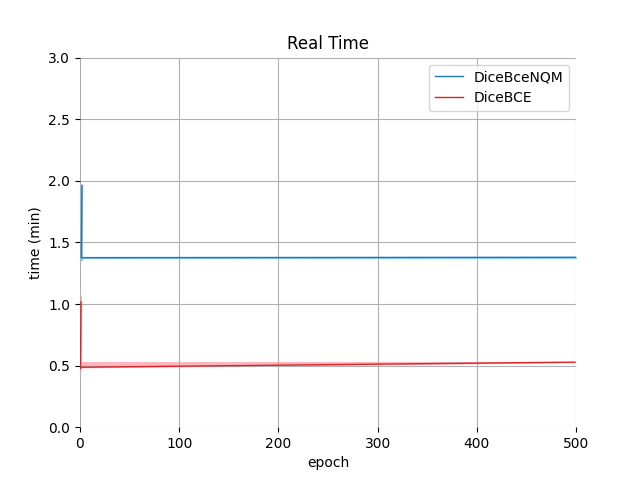
\includegraphics[width=\linewidth]{Graphics/Experiments/3.1.2_realTime_with_error_.png}
    \end{minipage} \hfill
    \begin{minipage}{0.49\textwidth}
        \centering
        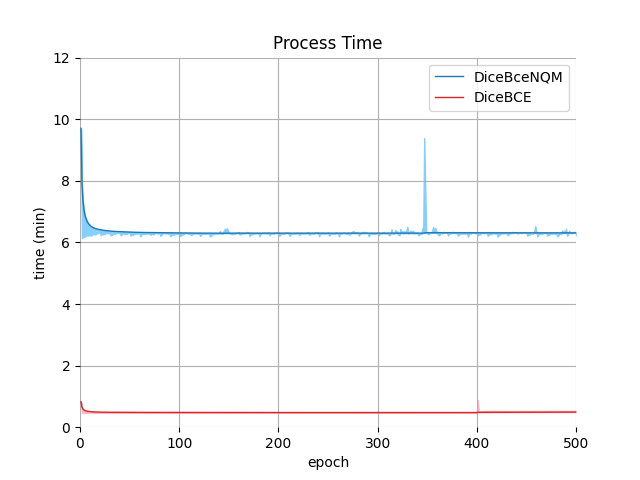
\includegraphics[width=\linewidth]{Graphics/Experiments/3.1.2_process_time_with_errors_.png}
    \end{minipage}
        \caption{Speed comparison between DiceBce and DiceBceNQM for real-time and process time. The average training times per epoch are shown in dark colors. The difference to the actual training times is shown in light colors behind the average. The DiceBceNQM takes much longer to train. The overall means for the real-time are 1.38 min and 0.49 min. The mean values for the process time are 6.33 min and 0.48 min.}
    \label{fig:DiceBCE+NQM:Pretrained:Speedcompare}
\end{figure}

Training on the DiceBceNQM with a stack size of 3 takes about 13.19 times as long as training on the DiceBCE alone and about 2.8 times as long in real time on the system we used (\autoref{experiments:intro:system}, as can be seen in \autoref{fig:DiceBCE+NQM:Pretrained:Speedcompare}). This is simply because with the stacksize, the number of predictions that need to be generated for the NQM is many times greater than without it. We mostly used a stacksize of 3 in our experiments. Therefore, we tested whether we could perform similarly by using pretrained models. To do this, we first trained a cohort of models on the Spike Hippocampus and not augmented datasets. Half of the cohort was trained for the entire 600 epochs on DiceBceNQM. The other half was pretrained for 500 epochs on DiceBCE and another 100 epochs on DiceBceNQM. The results are given in \autoref{tab:3.1.2:DiceBCE+NQM:Pretrained}. The pretrained models are continuously approximately as good as those fully trained on the DiceBceNQM. This is true for the models trained on augmented datasets and those trained on not augmented datasets. The one trained on the non-augmented dataset tends to get a little worse, but compared to the one trained on only 500 epochs \autoref{tab:03.1.1:DiceBCE+NQM_vs_DiceBCE_on_Spike}, both are better on the spike datasets and similar as good on the non-augmented one. Especially for those trained on the sparsely augmented dataset (Spike 0.01), the pretrained performs better rather than worse. 

The equivalence of these training methods is further emphasized when we look at the accumulations of the differences between pretrained and fully trained models for the entire cohort we trained for Dice: The maximum delta was $+ 0.037$, the sum of deltas was $-0.002$, the mean of the absolute deltas was $0.007$, the mean of signed deltas between these two groups was smaller in amount than $0.001$, up to these levels of accuracy. Each for the differences between the two models from the different groups trained on the same datasets (as shown as $\pm$ in the table).
\begin{table}[H]
    \centering
    \begin{tabular}{cl!{\vrule width 1.3pt}llllll}
        \toprule
        \multicolumn{2}{c!{\vrule width 1.3pt}}{model} &
        \multicolumn{5}{c}{\textbf{test dataset} (Dice $\uparrow$)}\\\midrule
        {\bfseries pretrained} & \textbf{train set} & original & Spike 1.0 & Spike 0.3 & Spike 0.2 & Spike 0.1 & Spike 0.01\\\midrule[1.3pt]
        % ---
        no  & original           & 0.881 & 0.662 & 0.812 & 0.811 & 0.858 & 0.881                            \\
        yes & original           & 0.879 & 0.639 -.02 & 0.802 -.01 & 0.801 -.01 & 0.857 & 0.879             \\\rowcolor{BG}
        no  & Spike 1.0          & 0.867 & 0.817 & 0.864 & 0.863 & 0.865 & 0.866                            \\\rowcolor{BG}
        yes & Spike 1.0          & 0.874 +.01 & 0.812 & 0.871 +.01 & 0.867 & 0.872 +.01 & 0.874 +.01        \\
        no  & Spike 0.3          & 0.874 & 0.750 & 0.853 & 0.859 & 0.870 & 0.875                            \\
        yes & Spike 0.3          & 0.872 & 0.757 +.01 & 0.858 +.01 & 0.859 & 0.868 & 0.872                  \\\rowcolor{BG}
        no  & Spike 0.2          & 0.878 & 0.751 & 0.843 & 0.863 & 0.869 & 0.878                            \\\rowcolor{BG}
        yes & Spike 0.2          & 0.879 & 0.727 -.02 & 0.830 -.01 & 0.862 & 0.869 & 0.879                  \\
        no  & Spike 0.1          & 0.875 & 0.754 & 0.849 & 0.860 & 0.869 & 0.876                            \\
        yes & Spike 0.1          & 0.875 & 0.735 -.02 & 0.842 -.01 & 0.855 -.01 & 0.866 & 0.875             \\\rowcolor{BG}
        no  & Spike 0.01         & 0.877 & 0.644 & 0.801 & 0.811 & 0.852 & 0.877                            \\\rowcolor{BG}
        yes & Spike 0.01         & 0.878 & 0.681 \textbf{+.04} & 0.816 +.01 & 0.833 +.02 & 0.861 +.01 & 0.877        \\\bottomrule
    \end{tabular}
    \caption{\textbf{Pretrained Models} (\autoref{experiments:03.1.2:backbone_hippo:pretrained}): Comparrison between pretrained models and full trained ones. For the pretrained models, we used the DiceBCE for the first 500 epochs, since it is faster, and trained after that on the DiceBceNQM for additional 100 epochs. For the not pretrained models we trained full 600 epochs on DiceBceNQM as baseline for the pretrained.\\
    The pretrained models are as good, as the full trained ones. Therefor they can be used to speed up training.}
    \label{tab:3.1.2:DiceBCE+NQM:Pretrained}  
\end{table}
\subsubsection{Hyperparameters}
\label{experiments:03.1.w:Hyperpatameters}

%%% was 03.1.3
\paragraph{stackSize}   
\label{experiments:03.1.3:backbone_hippo:stackSize}

In our experiments so far, we have used a \textit{stacksize} ($N$) of 3 for the DiceBceNQM, as defined in \autoref{eq:02.1:DiceBceNQM}. This seemed sufficient so far since different stack sizes had no effect when tested on not augmented data only \autoref{experiments:02.0:intro}. We want to test if these results also hold for augmented data. Nevertheless, training with the DiceBceNQM and a stacksize of 3 already takes about 2.8 times the real-time and 13.19 times the process time compared to the DiceBCE (\autoref{fig:DiceBCE+NQM:Pretrained:Speedcompare}). We trained a cohort of models on a stacksize of 6 but only on 3 spike datasets. We had to reduce the batch size to 16 because there was not enough VRAM for that large stacksize. Therefore, the models with a stacksize of 3, which we used for comparison, are also trained with a batch size of 16. The results can be seen in \autoref{tab:3.1.3:higherStacksize}. As one can see, there is no positive or negative effect of increasing the stacksize.

Since increasing the stacksize had no effect, we also tested whether a stacksize of 2 would be sufficient and, therefore, cheaper in terms of computation. This experiment was done later on a pretrained model with the stacksize we used elsewhere. As seen in \autoref{tab:3.1.3:smallerStacksize}, it does not worsen the results. Therefore, a stacksize of 2 can be considered sufficient or better, especially concerning the non-enlarged dataset. Unfortunately, this experiment was carried out very late, so our other experiments are still done on stacksize 3.
% Aggregated values are given in \autoref{tab:3.1.3:stackSize_aggregated}
\iftable
\begin{table}[H]
    \centering
    \begin{tabular}{cl!{\vrule width 1.3pt}llllll}
        \toprule
        \multicolumn{2}{c!{\vrule width 1.3pt}}{model} &
        \multicolumn{5}{c}{\textbf{test dataset} (Dice $\uparrow$)}\\\midrule
        {\bfseries Stacksize} & \textbf{train set} & original & Spike 1.0 & Spike 0.3 & Spike 0.2 & Spike 0.1 & Spike 0.01\\\midrule[1.3pt]
        % ---
        3 & original    & 0.881 & 0.611 & 0.798 & 0.799 & 0.856 & 0.881\\\rowcolor{BG}
        3 & Spike 0.3   & 0.878 & 0.782 & 0.868 & 0.863 & 0.873 & 0.877\\\rowcolor{BG}
        6 & Spike 0.3   & 0.880 & 0.788 +.01 & 0.864 & 0.865 & 0.875 & 0.879\\
        3 & Spike 0.2   & 0.876 & 0.728 & 0.832 & 0.860 & 0.868 & 0.876\\
        6 & Spike 0.2   & 0.879 & 0.743 +.02 & 0.839 +.01 & 0.862 & 0.867 & 0.879\\\rowcolor{BG}
        3 & Spike 0.1   & 0.880 & 0.753 & 0.856 & 0.862 & 0.875 & 0.880\\\rowcolor{BG}
        6 & Spike 0.1   & 0.877 & 0.738 -.02 & 0.848 -.01 & 0.859 & 0.870 -.01 & 0.877\\\bottomrule
    \end{tabular}
    \caption{\textbf{Higher Stacksize} (\autoref{experiments:03.1.3:backbone_hippo:stackSize}): Comparrison between stacksize 3 and stacksize 6. Model from first line is traind on Dice BCE for comparison. For the other models here, the trainloss is the DiceBceNQM, but with diffrent stackSize.\\
    A higher stacksize does not take any effekt, even though it is very expensive in computation time. All models are trained with a batchsize of 16, since the VRAM need with a stacksize of 6 was to high otherwise.}
    \label{tab:3.1.3:higherStacksize}
\end{table}

\begin{table}[H]
    \centering
    \begin{tabular}{cl!{\vrule width 1.3pt}llllll}
        \toprule
        \multicolumn{2}{c!{\vrule width 1.3pt}}{model} &
        \multicolumn{5}{c}{\textbf{test dataset} (Dice $\uparrow$)}\\\midrule
        {\bfseries Stacksize} & \textbf{train set} & original & Spike 1.0 & Spike 0.3 & Spike 0.2 & Spike 0.1 & Spike 0.01\\\midrule[1.3pt]
        % ---
        3 & original        & 0.881 & 0.662 & 0.812 & 0.811 & 0.858 & 0.881                           \\
        2 & original        & 0.882 & 0.645 -.02 & 0.801 -.01 & 0.809 & 0.853 -.01 & 0.883            \\\rowcolor{BG}
        3 & Spike1.0  & 0.867 & 0.817 & 0.864 & 0.863 & 0.865 & 0.866                           \\\rowcolor{BG}
        2 & Spike1.0  & 0.872 +.01 & 0.825 +.01 & 0.867 & 0.867 & 0.870 +.01 & 0.872 +.01       \\
        3 & Spike0.3  & 0.874 & 0.750 & 0.853 & 0.859 & 0.870 & 0.875                           \\
        2 & Spike0.3  & 0.876 & 0.756 +.01 & 0.854 & 0.858 & 0.871 & 0.875                      \\\rowcolor{BG}
        3 & Spike0.2  & 0.878 & 0.751 & 0.843 & 0.863 & 0.869 & 0.878                           \\\rowcolor{BG}
        2 & Spike0.2  & 0.878 & 0.737 -.01 & 0.835 -.01 & 0.861 & 0.864 -.01 & 0.878            \\
        3 & Spike0.1  & 0.875 & 0.754 & 0.849 & 0.860 & 0.869 & 0.876                           \\
        2 & Spike0.1  & 0.880 +.01 & 0.765 +.01 & 0.858 +.01 & 0.865 +.01 & 0.875 +.01 & 0.880  \\\rowcolor{BG}
        3 & Spike0.01 & 0.877 & 0.644 & 0.801 & 0.811 & 0.852 & 0.877                           \\\rowcolor{BG}
        2 & Spike0.01 & 0.881 & 0.659 +.02 & 0.816 +.01 & 0.823 +.01 & 0.861 +.01 & 0.881       \\\bottomrule
    \end{tabular}
    \caption{\textbf{Smaller Stacksize} (\autoref{experiments:03.1.3:backbone_hippo:stackSize}): Comparrison between stacksize 3 and stacksize 2. Models are trained on the DiceBceNQM, but with diffrent stackSize.\\
    A stacksize of 2 is as good as a stacksize of 3, even though a higher stacksize is more expensive in computation time and VRAM.}
    \label{tab:3.1.3:smallerStacksize}
\end{table}
\fi

%%% alpha was 03.1.4  %%%
\paragraph{alpha}   
\label{experiments:03.1.4:backbone_hippo:alpha}
Here, we have checked whether it makes a difference if the proportion of the NQM in the total DiceBceNQM is varied. To do this, we added the parameter alpha ($\alpha$) so that the previous DiceBceNQM corresponds to $\alpha=1.0$, i.e:

\begin{align}
    \text{DiceBce-$\alpha$NQM} &:= 1 - \mathrm{Dice} + \mathrm{Bce} + {\color{red}\alpha}\cdot\mathrm{NQM}
\end{align}

Where the NQM is defined as in \autoref{eq:02.1:Only_NQM}. We have trained two cohorts. One with halved and one with doubled $\alpha$. We trained all models for 100 epochs each on a pretrained model, as in \autoref{experiments:03.1.2:backbone_hippo:pretrained}. The results in \autoref{tab:3.1.4:alpha} shows that a double $\alpha$ further increases the robustness. This is especially true when training on the less augmented dataset, and there is no degradation when training on not augmented data.

Beyond these variations on the same loss function with different alphas, we tested other loss functions that should converge more strongly and penalize higher NQM values more strongly. We will look at this in the following.
\iffalse
\begin{table}[H]
    \centering
    \begin{tabular}{cl!{\vrule width 1.3pt}llllll}
        \toprule
        \multicolumn{2}{c!{\vrule width 1.3pt}}{model} &
        \multicolumn{5}{c}{\textbf{test dataset} (Dice $\uparrow$)}\\\midrule
        \textbf{alpha} & \textbf{train set} & original & spike 1.0 & spike 0.3 & spike 0.2 & spike 0.1 & spike 0.01\\\midrule[1.3pt]
        % ---
        1.0 & original     & 0.881 & 0.662 & 0.812 & 0.811 & 0.858 & 0.881\\
        0.5 & original     & 0.881 & 0.636 \textbf{-.03} & 0.808 & 0.790 -.02 & 0.850 -.01 & 0.880\\
        2.0 & original     & 0.879 & 0.672 +.01 & 0.815 & 0.821 +.01 & 0.858 & 0.879\\\rowcolor{BG}
        1.0 & Spike 1.0    & 0.867 & 0.817 & 0.864 & 0.863 & 0.865 & 0.866\\\rowcolor{BG}
        0.5 & Spike 1.0    & 0.873 +.01 & 0.805 -.01 & 0.868 & 0.866 & 0.871 +.01 & 0.874 +.01\\\rowcolor{BG}
        2.0 & Spike 1.0    & 0.869 & 0.814 & 0.866 & 0.863 & 0.868 & 0.869\\
        1.0 & Spike 0.3    & 0.874 & 0.750 & 0.853 & 0.859 & 0.870 & 0.875\\
        0.5 & Spike 0.3    & 0.876 & 0.745 -.01 & 0.854 & 0.862 & 0.870 & 0.877\\
        2.0 & Spike 0.3    & 0.875 & 0.771 +.02 & 0.858 +.01 & 0.861 & 0.871 & 0.875\\\rowcolor{BG}
        1.0 & Spike 0.2    & 0.878 & 0.751 & 0.843 & 0.863 & 0.869 & 0.878\\\rowcolor{BG}
        0.5 & Spike 0.2    & 0.878 & 0.739 -.01 & 0.842 & 0.863 & 0.867 & 0.878\\\rowcolor{BG}
        2.0 & Spike 0.2    & 0.878 & 0.738 -.01 & 0.835 -.01 & 0.862 & 0.870 & 0.878\\
        1.0 & Spike 0.1    & 0.875 & 0.754 & 0.849 & 0.860 & 0.869 & 0.876\\
        0.5 & Spike 0.1    & 0.879 & 0.762 +.01 & 0.850 & 0.860 & 0.875 +.01 & 0.879\\
        2.0 & Spike 0.1    & 0.874 & 0.759 +.01 & 0.846 & 0.856 & 0.870 & 0.875\\\rowcolor{BG}
        1.0 & Spike 0.01   & 0.877 & 0.644 & 0.801 & 0.811 & 0.852 & 0.877\\\rowcolor{BG}
        0.5 & Spike 0.01   & 0.880 & 0.639 -.01 & 0.808 +.01 & 0.806 -.01 & 0.856 & 0.880\\\rowcolor{BG}
        2.0 & Spike 0.01   & 0.879 & 0.686 \textbf{+.04} & 0.826 +.02 & 0.846 \textbf{+.03} & 0.865 +.01 & 0.879\\\bottomrule
    \end{tabular}
    \caption{\textbf{DiceBceNQM with different alphas} (\autoref{experiments:03.1.4:backbone_hippo:alpha}): The standard we used for all other experiments for $\alpha$ is $1.0$. So the diffrences shown are with respect to the models trained with $\alpha=1.0$ on the same train dataset.\\ 
    An $\alpha$ of $2.0$ leads to more robust models here.}
    \label{tab:3.1.4:alpha}
\end{table}
\fi
\subsubsection{Non-Linear NQM Losses}
\label{experiments:03.1.x:FurtherNQMLosses}
\begin{figure}[h!]
    \centering
        \begin{minipage}{0.49\textwidth}
        \centering
        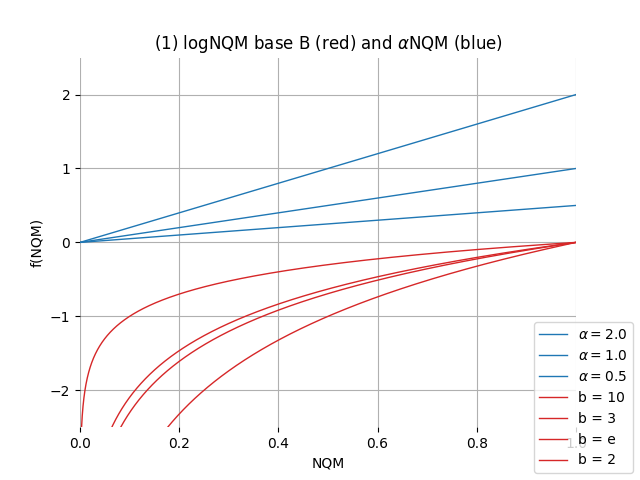
\includegraphics[width=\linewidth]{Graphics/Experiments/3.1_alphas_logs.png}
    \end{minipage} \hfill
    \begin{minipage}{0.49\textwidth}
        \centering
        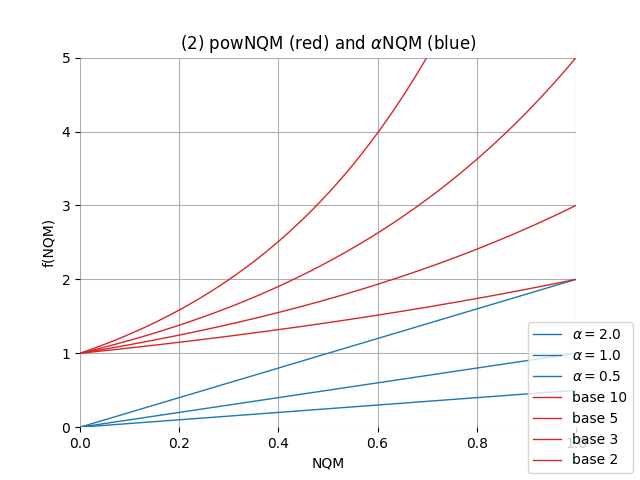
\includegraphics[width=\linewidth]{Graphics/Experiments/3.1_alphas_pow.png}
    \end{minipage}
    \begin{minipage}{0.49\textwidth}
        \centering
        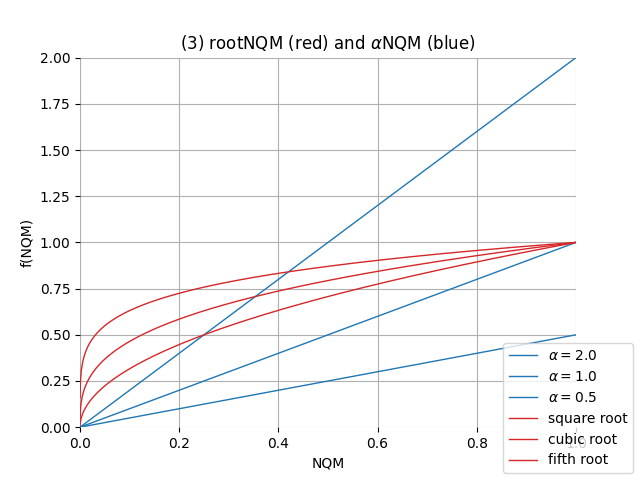
\includegraphics[width=\linewidth]{Graphics/Experiments/3.1_alphas_root.png}
    \end{minipage}
    \caption{Non-linear functions we used for NQM losses (red), to test, if they perform similar or better in comparison to the linar DiceBce-$\alpha$NQM (blue). The order in the legend within a color also corresponds to the order in which the functions are superimposed in the plot. In the range of the NQM $(0, 1)$.}
    \label{fig:furtherFunctionsForNQM}
\end{figure}

Since we have seen promising results with the linear NQM alone and with different alphas in terms of robustness to augmented data, we decided to test whether other loss functions with NQM could lead to similar or even better results. On the one hand, we chose functions that might converge more strongly because they weight higher NQM values more strongly than linear functions (logarithm, power, and root functions) or might converge similarly well. Examples of these can be seen in \autoref{fig:furtherFunctionsForNQM}. Each is compared to the linear case for the three slopes we tested in \autoref{experiments:03.1.4:backbone_hippo:alpha} (blue). 

For our experiments here, we used a pretrained model that we first trained for 500 epochs on the DiceBCE. Then, we trained this model for another 100 epochs on the corresponding loss.
We trained a cohort for each loss to be tested. Each cohort was trained on the original and with spikes augmented hippocampus datasets because this is where we have seen the clearest results with the DiceBceNQM so far. So, there are six datasets in total and one model for each dataset in each cohort. For the comparisons here, we assumed the DiceBceNQM, i.e., corresponding to $\alpha=1.0$, and trained one cohort accordingly.

%%% log NQM %%%
\paragraph{Logarithmic NQM Loss}
\label{experiments:03.1.5:backbone_hippo:logNQM}
Since the NQM assumes a value between 0 and 1, and the logarithm (log) falls to 0 faster than linearly, particularly small values are rewarded very highly with the log, i.e., the total loss is greatly reduced. This means that the NQM's share of the total loss is no longer capped (unlike in the other cases). Since this negative growth occurs at different rates with different bases, we tested several log functions with different bases. Therefore, the logNQM base B is defined as:

\begin{align}
    \text{logNQM base B} &:= 1 - \mathrm{Dice} + \mathrm{Bce} + {\color{red}\log_B}\mathrm{NQM}
\end{align}

We decided to test bases 2, e, 3, and 10. So, we trained a total of 4 cohorts on the logNQM. As seen in \autoref{tab:3.1.5:logNQM}, using a logarithmic NQM leads to mixed results compared to the linear NQM. In particular, on the original dataset, the logNQM consistently leads to a degradation of up to 9 points on the dice. On the other hand, when training on the augmented dataset, the logNQM results in a slight improvement of up to 3 points. \autoref{tab:3.1.5:logNQM_aggregated} shows various aggregations of the improvements and deteriorations in scores for each cohort. Again, there is an overall almost neutral but negative mean on the signed differences and a range shift clearly into the negative.\\\
Our implementation of the NQM with this loss could not further improve the robustness. 
% \todo{evt. Fehler bei den Labels zeigen, die mit höherer Base schlimmer werden ... war hier relativ klar zu sehen, bei manchen samples ... dann Verknüpfung nach onlyNQM, weil vermutlich ähnlihcer grund ... wobei hier der Dice immernoch über die 100 epochen gefallen ist.}
\iftable
\begin{table}[H]
    \centering
    \begin{tabular}{ll!{\vrule width 1.3pt}llllll}
        \toprule
        \multicolumn{2}{c!{\vrule width 1.3pt}}{model} &
        \multicolumn{5}{c}{\textbf{test dataset} (Dice $\uparrow$)}\\\midrule
        {\bfseries train loss} & \textbf{train set} & original & spike 1.0 & spike 0.3 & spike 0.2 & spike 0.1 & spike 0.01\\\midrule[1.3pt]
        % ---
        DiceBceNQM      & original     & 0.881 & 0.662 & 0.812 & 0.811 & 0.858 & 0.881\\
        powNQM base 3   & original     & 0.877 & 0.616 \textbf{-.05} & 0.809 & 0.793 -.02 & 0.853 -.01 & 0.877\\\rowcolor{BG}
        DiceBceNQM      & Spike 1.0    & 0.867 & 0.817 & 0.864 & 0.863 & 0.865 & 0.866\\\rowcolor{BG}
        powNQM base 3   & Spike 1.0    & 0.867 & 0.815 & 0.863 & 0.859 & 0.865 & 0.867\\
        DiceBceNQM      & Spike 0.3    & 0.874 & 0.750 & 0.853 & 0.859 & 0.870 & 0.875\\
        powNQM base 3   & Spike 0.3    & 0.875 & 0.768 +.02 & 0.857 & 0.861 & 0.873 & 0.875\\\rowcolor{BG}
        DiceBceNQM      & Spike 0.2    & 0.878 & 0.751 & 0.843 & 0.863 & 0.869 & 0.878\\\rowcolor{BG}
        powNQM base 3   & Spike 0.2    & 0.874 & 0.730 -.02 & 0.832 -.01 & 0.855 -.01 & 0.863 -.01 & 0.874\\
        DiceBceNQM      & Spike 0.1    & 0.875 & 0.754 & 0.849 & 0.860 & 0.869 & 0.876\\
        powNQM base 3   & Spike 0.1    & 0.879 & 0.749 -.01 & 0.855 +.01 & 0.862 & 0.871 & 0.878\\\rowcolor{BG}
        DiceBceNQM      & Spike 0.01   & 0.877 & 0.644 & 0.801 & 0.811 & 0.852 & 0.877\\\rowcolor{BG}
        powNQM base 3   & Spike 0.01   & 0.879 & 0.668 +.02 & 0.815 +.01 & 0.832 +.02 & 0.861 +.01 & 0.879\\\bottomrule
    \end{tabular}
    \caption{\textbf{powNQM} (\autoref{experiments:03.1.6:backbone_hippo:powNQM}): Linear DiceBceNQM for comparisson. Only diffrences größer round $\pm$0.01 are shown (always in comparison to row above)\\
    Overall, powNQM base 3 does not lead to any improvement.}
    \label{tab:3.1.6:powNQM}
\end{table}
\fi

\begin{table}[h!]
    \centering
    \begin{tabular}{|c|l|l|l|l|}
        \hline
        \bfseries logNQM base & mean on signed & mean on absolute & sum on absolute & range\\\hline
        % ---
        2   & -0.0004 & 0.0063 & 0.226 & ( -0.053, +0.030)\\
        e   & -0.0011 & 0.0076 & 0.275 & ( -0.038, +0.033)\\
        3   & -0.0031 & 0.0074 & 0.266 & ( -0.086, +0.014)\\
        10  & -0.0011 & 0.0056 & 0.2   & ( -0.037, +0.024)\\\hline
        % ---
    \end{tabular}
    \caption{Aggregations over the improvements$(+)$ and deteriorations$(-)$, using the logNQM losses compared to the DiceBceNQM on Dice. All values of the experiments used for this Aggregations: \autoref{tab:3.1.5:logNQM}}
    \label{tab:3.1.5:logNQM_aggregated}
\end{table}


%%% pow NQM %%%
\paragraph{Power NQM Loss}
\label{experiments:03.1.6:backbone_hippo:powNQM}
As one can see in \autoref{fig:furtherFunctionsForNQM}, the power function is the opposite of the log function. While the log function rewards particularly small values in the range $(0,1)$ more, the power function punishes exceptionally high values. We have implemented this loss due to the range of the NQM in $(0,1)$ by choosing a constant base and placing the NQM in the exponent. Conversely, when using the NQM to the pow of something, growth is slower than linear in this interval.
Therefore, the powNQM base is defined as B:

\begin{align}
    \text{powNQM base B} &:= 1 - \mathrm{Dice} + \mathrm{Bce} + {\color{red} \mathrm{B}}^\mathrm{NQM}
\end{align}

Here, we have trained a cohort on base 3. The results are shown in \autoref{tab:3.1.6:powNQM}. The aggregated improvements and degradations are given in \autoref{tab:3.1.6:powNQM_aggregated}. As can be seen, the powNQM hardly leads to any change, which is evident when looking at the corresponding base function in \autoref{experiments:03.1.x:FurtherNQMLosses}, since the pow function with base 3 behaves almost linearly here. However, the tendency here is similar to logNQM, that models trained on the not augmented data perform worse on the augmented data. The reverse does not seem to be the case.
Therefore, it might be interesting to test a higher base again, but this was not done in the context of this work \autoref{future_work}.

\begin{table}[h!]
    \centering
    \begin{tabular}{|c|l|l|l|l|}
        \hline
        \bfseries pow NQM base & mean on signed & mean on absolute & sum on absolute & range\\\hline
        % ---
        3 & -0.0008 & 0.0073 & 0.263 & (-0.046, +0.024)\\\hline
        % ---
    \end{tabular}
    \caption{Agreggations over the improvements$(+)$ and deteriorations$(-)$, using the powNQM compared to the DiceBceNQM on Dice. All values of the experiments used for theses Aggregations: \autoref{tab:3.1.6:powNQM}}
    \label{tab:3.1.6:powNQM_aggregated}
\end{table}

\iftable
\begin{table}[H]
    \centering
    \begin{tabular}{ll!{\vrule width 1.3pt}llllll}
        \toprule
        \multicolumn{2}{c!{\vrule width 1.3pt}}{model} &
        \multicolumn{5}{c}{\textbf{test dataset} (Dice $\uparrow$)}\\\midrule
        {\bfseries train loss} & \textbf{train set} & original & spike 1.0 & spike 0.3 & spike 0.2 & spike 0.1 & spike 0.01\\\midrule[1.3pt]
        % ---
        DiceBceNQM     & original     & 0.881 & 0.662 & 0.812 & 0.811 & 0.858 & 0.881\\
        logNQM base 2  & original     & 0.878 & 0.609 \textbf{-.05} & 0.800 -.01 & 0.797 -.01 & 0.847 -.01 & 0.877\\
        logNQM base e  & original     & 0.879 & 0.624 \textbf{-.04} & 0.803 -.01 & 0.795 -.02 & 0.848 -.01 & 0.879\\
        logNQM base 3  & original     & 0.881 & 0.576 \textbf{-.09} & 0.797 -.02 & 0.789 -.02 & 0.842 -.02 & 0.881\\
        logNQM base 10 & original     & 0.882 & 0.625 \textbf{-.04} & 0.810 & 0.805 -.01 & 0.854 & 0.882\\\rowcolor{BG}
        DiceBceNQM     & Spike 1.0    & 0.867 & 0.817 & 0.864 & 0.863 & 0.865 & 0.866\\\rowcolor{BG}
        logNQM base 2  & Spike 1.0    & 0.869 & 0.813 & 0.865 & 0.864 & 0.867 & 0.869\\\rowcolor{BG}
        logNQM base e  & Spike 1.0    & 0.873 +.01 & 0.822 +.01 & 0.869 +.01 & 0.868 +.01 & 0.871 +.01 & 0.872 +.01\\\rowcolor{BG}
        logNQM base 3  & Spike 1.0    & 0.870 & 0.831 +.01 & 0.866 & 0.866 & 0.869 & 0.870\\\rowcolor{BG}
        logNQM base 10 & Spike 1.0    & 0.870 & 0.811 -.01 & 0.864 & 0.864 & 0.867 & 0.870\\
        DiceBceNQM     & Spike 0.3    & 0.874 & 0.750 & 0.853 & 0.859 & 0.870 & 0.875\\
        logNQM base 2  & Spike 0.3    & 0.875 & 0.747 & 0.852 & 0.859 & 0.869 & 0.874\\
        logNQM base e  & Spike 0.3    & 0.878 & 0.783 \textbf{+.03} & 0.861 +.01 & 0.864 +.01 & 0.874 & 0.878\\
        logNQM base 3  & Spike 0.3    & 0.877 & 0.756 +.01 & 0.859 +.01 & 0.862 & 0.873 & 0.877\\
        logNQM base 10 & Spike 0.3    & 0.877 & 0.774 +.02 & 0.863 +.01 & 0.862 & 0.872 & 0.877\\\rowcolor{BG}
        DiceBceNQM     & Spike 0.2    & 0.878 & 0.751 & 0.843 & 0.863 & 0.869 & 0.878\\\rowcolor{BG}
        logNQM base 2  & Spike 0.2    & 0.879 & 0.752 & 0.844 & 0.862 & 0.869 & 0.879\\\rowcolor{BG}
        logNQM base e  & Spike 0.2    & 0.873 -.01 & 0.725 \textbf{-.03} & 0.826 -.02 & 0.857 -.01 & 0.862 -.01 & 0.872 -.01\\\rowcolor{BG}
        logNQM base 3  & Spike 0.2    & 0.879 & 0.741 -.01 & 0.837 -.01 & 0.862 & 0.868 & 0.879\\\rowcolor{BG}
        logNQM base 10 & Spike 0.2    & 0.877 & 0.735 -.02 & 0.836 -.01 & 0.857 -.01 & 0.864 -.01 & 0.877\\
        DiceBceNQM     & Spike 0.1    & 0.875 & 0.754 & 0.849 & 0.860 & 0.869 & 0.876\\
        logNQM base 2  & Spike 0.1    & 0.876 & 0.744 -.01 & 0.847 & 0.860 & 0.869 & 0.877\\
        logNQM base e  & Spike 0.1    & 0.877 & 0.746 -.01 & 0.850 & 0.854 -.01 & 0.871 & 0.877\\
        logNQM base 3  & Spike 0.1    & 0.880 +.01 & 0.751 & 0.851 & 0.865 +.01 & 0.874 +.01 & 0.880\\
        logNQM base 10 & Spike 0.1    & 0.876 & 0.742 -.01 & 0.842 -.01 & 0.857 & 0.869 & 0.875\\\rowcolor{BG}
        DiceBceNQM     & Spike 0.01   & 0.877 & 0.644 & 0.801 & 0.811 & 0.852 & 0.877\\\rowcolor{BG}
        logNQM base 2  & Spike 0.01   & 0.878 & 0.674 \textbf{+.03} & 0.830 \textbf{+.03} & 0.835 +.02 & 0.857 +.01 & 0.878\\\rowcolor{BG}
        logNQM base e  & Spike 0.01   & 0.877 & 0.644 & 0.809 +.01 & 0.824 +.01 & 0.852 & 0.877\\\rowcolor{BG}
        logNQM base 3  & Spike 0.01   & 0.878 & 0.627 -.02 & 0.798 & 0.803 -.01 & 0.851 & 0.877\\\rowcolor{BG}
        logNQM base 10 & Spike 0.01   & 0.876 & 0.652 +.01 & 0.811 +.01 & 0.816 & 0.848 & 0.876\\\bottomrule
    \end{tabular}
    \caption{\textbf{logNQM for diffrent bases} (\autoref{experiments:03.1.5:backbone_hippo:logNQM}): For bases 2, e, 3 and 10. linear DiceBceNQM as comparison. Only diffrences bigger round $\pm$.01 are shown (always in comparison to the top row of the block, the model trained on the DiceBce-NQM).\\Overall, the logNQM does not lead to any further improvement in robustness here.}
    \label{tab:3.1.5:logNQM}
\end{table}
\fi

%%% sqrt NQM %%%
\paragraph{Square Root NQM Loss}
\label{experiments:03.1.7:backbone_hippo:sqrtNQM}
As seen in \autoref{fig:furtherFunctionsForNQM}, the root function in the interval $(0,1)$ decays to zero, similarly to the logarithmic function. However, they do not try to reach $-\infty$ but fall to zero. This means that very small values in the root functions have very little weight. At the same time, there is a low upper bound of one that the function can assume. That way, the NQM's share of the total loss is limited, in contrast to the logarithmic function in particular, which has no limit at all, but also to the power functions, where the upper bound corresponds to the base and grows accordingly. We tested the square root function since this shows the described behavior most clearly. 
Therefore, the sqrtNQM is defined as:

\begin{align}
    \text{sqrtNQM} &:= 1 - \mathrm{Dice} + \mathrm{Bce} + \sqrtRed{\text{NQM}} 
\end{align}

Again, we trained a cohort on this loss. The results are shown in \autoref{tab:3.1.7:sqrtNQM}. The aggregated improvements and deteriorations are shown in \autoref{tab:3.1.7:sqrtNQM_aggregated}. Again, there does not appear to be much difference from the linear implementation. There may be a slight improvement in the minimally augmented dataset (spike 0.01). At the same time, there is no degradation in the not augmented dataset. This is different for logNQM and powNQM. This makes the sqrtNQM a candidate for speeding up the approach. Further experiments with domain shifts and other datasets would be interesting, too. Possibly also as cubic root or a mixture of pow and root function, in the sense of powNQM -1 + sqrtNQN (\autoref{future_work}). 

\begin{table}[h!]
    \centering
    \begin{tabular}{|c|l|l|l|l|}
        \hline
        \bfseries sqrt NQM & mean on signed & mean on absolute & sum on absolute & range\\\hline
        % ---
        & -0.0023 & 0.0084 & 0.304 & (-0.026, +0.033)\\\hline
        % ---
    \end{tabular}
    \caption{Agreggations over the improvements$(+)$ and deteriorations$(-)$, using the sqrtNQM compared to the DiceBceNQM on Dice. All values of the experiments used for theese Aggregations: \autoref{tab:3.1.7:sqrtNQM}}
    \label{tab:3.1.7:sqrtNQM_aggregated}
\end{table}
\iftable
\begin{table}[H]
    \centering
    \begin{tabular}{ll!{\vrule width 1.3pt}llllll}
        \toprule
        \multicolumn{2}{c!{\vrule width 1.3pt}}{model} &
        \multicolumn{5}{c}{\textbf{test dataset} (Dice $\uparrow$)}\\\midrule
        {\bfseries train loss} & \textbf{train set} & original & spike 1.0 & spike 0.3 & spike 0.2 & spike 0.1 & spike 0.01\\\midrule[1.3pt]
        % ---
        DiceBceNQM & original       & 0.881 & 0.662 & 0.812 & 0.811 & 0.858 & 0.881\\
        sqrtNQM    & original       & 0.875 -.01 & 0.694 \textbf{+.03} & 0.816 & 0.811 & 0.852 -.01 & 0.875 -.01\\\rowcolor{BG}
        DiceBceNQM & Spike 1.0      & 0.867 & 0.817 & 0.864 & 0.863 & 0.865 & 0.866\\\rowcolor{BG}
        sqrtNQM    & Spike 1.0      & 0.868 & 0.803 -.01 & 0.864 & 0.861 & 0.866 & 0.868\\
        DiceBceNQM & Spike 0.3      & 0.874 & 0.750 & 0.853 & 0.859 & 0.870 & 0.875\\
        sqrtNQM    & Spike 0.3      & 0.873 & 0.758 +.01 & 0.854 & 0.858 & 0.868 & 0.872\\\rowcolor{BG}
        DiceBceNQM & Spike 0.2      & 0.878 & 0.751 & 0.843 & 0.863 & 0.869 & 0.878\\\rowcolor{BG}
        sqrtNQM    & Spike 0.2      & 0.870 -.01 & 0.731 -.02 & 0.825 -.02 & 0.853 -.01 & 0.860 -.01 & 0.870 -.01\\
        DiceBceNQM & Spike 0.1      & 0.875 & 0.754 & 0.849 & 0.860 & 0.869 & 0.876\\
        sqrtNQM    & Spike 0.1      & 0.868 -.01 & 0.728 -.03 & 0.836 -.01 & 0.847 -.01 & 0.859 -.01 & 0.868 -.01\\\rowcolor{BG}
        DiceBceNQM & Spike 0.01     & 0.877 & 0.644 & 0.801 & 0.811 & 0.852 & 0.877\\\rowcolor{BG}
        sqrtNQM    & Spike 0.01     & 0.876 & 0.677 \textbf{+.03} & 0.811 +.01 & 0.827 +.02 & 0.855 & 0.876\\\bottomrule
    \end{tabular}
    \caption{\textbf{sqrtNQM} (\autoref{experiments:03.1.7:backbone_hippo:sqrtNQM}): Linear DiceBceNQM for comparisson. Only diffrences größer round $\pm$0.01 are shown (always in comparison to row above)\\
    Overall, the sqrtNQM leads to another small improvement.}
    \label{tab:3.1.7:sqrtNQM}
\end{table}
\fi
\iffalse
%%% SD as weights in BCE .... I can not figure out anymore, what this loss acctually was about ... looks, like I stuck in debugging and tried to implement it that way, it is discribed here, but the acctual loss, used in the experiment was only Bce(SD) for NQM ... so only logarithmically weighted SD in normal NQM .... should be of no intrest so far ...%%%
\paragraph{SD as weights in BCE}
\label{experiments:03.1.8:backbone_hippo:stdd BCE}
.\\\note{XXX HIER WEITER XXX Wie Paragraphs above XXX}

Bis jetzt haben wir für alle Versuche den NQM zum loss hinzugefügt, wie in \autoref{eq:02.1:Only_NQM} definiert. Der NQM besteht dabei aus zwei Teilen, der Standartabweichung (SD) und dem Mean. Dabei wird zur Bildung des NQM die SD mit dem mean normalisiert. Der Bce ist hier ähnlich zum NQM, auch dieser wird mit dem mean normalisiert. Insofern ist es naheliegend, zu testen, ob es einen Unterschied macht, den NQM und den Bce vor der Normalisierung zusammenzufassen. Also, den Bce mit dem SD zu gewichten und anschließend zu normalisieren. Für $N$ (stacksize) different predictions $x_i$ of an NCA for the same image volume $x$, with the target or groundthruth label $y$ and the image size $M$:

\begin{align*}
    \text{Dice-SDBce} &:= 1 - \mathrm{Dice} + {\color{red}\mathrm{SDBce}}\\[10pt]
    \text{SDBce}      &:=\min\left(1, \quad \frac{\sum_{n=1}^M (\text{SDBce}_n) +1} {\sum_{n=1}^M (\mu_n) +1}\right)\\[10pt]
    \text{SDBce}      &:=  - SD_n \cdot [y_n \cdot \log v_n + (1-y_n) \cdot \log (1-v_n)]\\[10pt]
    SD                &:= \sqrt{\frac{\sum^N_{i=1}(v_i-\mu)^2}  {N} + \varepsilon}\\[10pt]
    \mu               &:= \frac{\sum^N_{i=1}v_i}  {N}
\end{align*}

Der mean($\mu$) wird also genau wie in \autoref{eq:02.1:Only_NQM} über dem output stack gebildet. Der BCE ist, wie in \autoref{methods:NCA:Models} aber ohne mean-normalisierung. Den SD haben wir hier, wie sonst den NQM, zusätzlich vor der gewichtung des Bce, auf das Intervall $(0,1)$ gecroped und um $\varepsilon$ ergänzt. For the same reason as in \autoref{experiments:02.2:diceBce+NQM}. Es wäre natürlich auch interessant zu sehen, ob es einen Performanceunterschied macht, hier nicht zu croppen \autoref{future_work}. 

 ... tatsächlich gleich gut, also möglicherweise $\mu$ -normalisierung nicht nötig.

\todo{XXX Evaluiere (explizit in schriftlaut) alle Augmentationen gemäß der Robustheit gegenüber 1) der performance, wenn Artefakte im Trainingssatz enthalten waren, wie auch, wenn diese nicht im Traingssatz enthalten waren. XXX}
XXX neue Tabelle drinn XXX

\begin{table}[h!]
    \centering
    \begin{tabular}{|l|l|l|l|l|}
        \hline
        \bfseries & mean on signed & mean on absolute & sum on absolute & range\\\hline
        % ---
        \bfseries SD & -0.0007 & 0.0049 & 0.178 & (-0.032, +0.017)\\\hline
        % ---
    \end{tabular}
    \caption{Agreggations over the improvements$(+)$ and deteriorations$(-)$, using the SD compared to the DiceBceNQM on Dice. All values of the experiments, used for this Aggregations: \autoref{tab:3.1.8:stddBCE}}
    \label{tab:3.1.8:stddBCE_aggregated}
\end{table}

Bereits in \autoref{experiments:02.0:intro} hatten wir auch 
\iftable
\begin{table}[H]
    \centering
    \begin{tabular}{ll!{\vrule width 1.3pt}llllll}
        \toprule
        \multicolumn{2}{c!{\vrule width 1.3pt}}{model} &
        \multicolumn{5}{c}{\textbf{test dataset} (Dice $\uparrow$)}\\\midrule
        {\bfseries train loss} & \textbf{train set} & original & spike 1.0 & spike 0.3 & spike 0.2 & spike 0.1 & spike 0.01\\\midrule[1.3pt]
        % ---
        Dice-SDBce   & original          & 0.881 & 0.662 & 0.812 & 0.811 & 0.858 & 0.881\\
        DiceBce + SD    & original          & 0.876 -.01 & 0.630 \textbf{-.03} & 0.804 -.01 & 0.798 -.01 & 0.851 -.01 & 0.877\\\rowcolor{BG}
        Dice-SDBce   & Spike1.0          & 0.867 & 0.817 & 0.864 & 0.863 & 0.865 & 0.866\\\rowcolor{BG}
        DiceBce + SD    & Spike1.0          & 0.870 & 0.819 & 0.867 & 0.867 & 0.869 & 0.870\\
        Dice-SDBce   & Spike0.3          & 0.874 & 0.750 & 0.853 & 0.859 & 0.870 & 0.875\\
        DiceBce + SD    & Spike0.3          & 0.875 & 0.767 +.02 & 0.856 & 0.860 & 0.870 & 0.874\\\rowcolor{BG}
        Dice-SDBce   & Spike0.2          & 0.878 & 0.751 & 0.843 & 0.863 & 0.869 & 0.878\\\rowcolor{BG}
        DiceBce + SD    & Spike0.2          & 0.879 & 0.744 -.01 & 0.839 & 0.865 & 0.874 +.01 & 0.879\\
        Dice-SDBce   & Spike0.1          & 0.875 & 0.754 & 0.849 & 0.860 & 0.869 & 0.876\\
        DiceBce + SD    & Spike0.1          & 0.876 & 0.742 -.01 & 0.853 & 0.860 & 0.872 & 0.876\\\rowcolor{BG}
        Dice-SDBce   & Spike0.01         & 0.877 & 0.644 & 0.801 & 0.811 & 0.852 & 0.877\\\rowcolor{BG}
        DiceBce + SD    & Spike0.01         & 0.880 & 0.648 & 0.806 +.01 & 0.803 -.01 & 0.855 & 0.880\\\bottomrule
    \end{tabular}
    \caption{\textbf{SD as weights in BCE} (\autoref{experiments:03.1.8:backbone_hippo:stdd BCE}: Linear DiceBceNQM as comparisson. Only diffrences größer round $\pm$0.01 are shown (always in comparison to row above)\\
    Der SD wird zunächst als gewichte für den Bce genommen, bevor, wie beim NQM mit dem mean normalisiert wird. Die Performance scheint aber (fast) gleich zu bleiben.}
    \label{tab:3.1.8:stddBCE}
\end{table}
\fi
\fi